\chapter{代数幾何と弦理論の発展的話題}
\label{ch:ch17}

\begin{chapterlead}
本編で学んだ概念を現代的な理論へつなげるための概観．
本章では，楕円曲線，ミラー対称性，幾何学的遷移，D ブレーンと導来圏，F 理論という五つの話題を取り上げ，
これまでに準備した道具（射影多様体，層とコホモロジー，Hodge 数，特異点解消，モジュライ空間）がどのように使われるかを見る．
各話題はそれ自体が一つの研究分野であり，ここでは証明よりも「何が主張されているか」と「どの道具が必要か」を重視する．予想や未解決の問題はそのように明記する．
最後に，さらに学ぶための道筋と文献を挙げる．
\end{chapterlead}

%======================================================================
\section{楕円曲線と物理}
%======================================================================

\subsection{楕円曲線の定義}

\begin{mydef}{楕円曲線}{ch17-elliptic-curve}
体 $k$ 上の\textbf{楕円曲線}とは，種数 $1$ の滑らかな射影代数曲線 $E$ と，$E$ 上の $k$ 有理点 $O$ の組 $(E,O)$ をいう．
\end{mydef}

$k=\C$ の場合，第13章で見たように $E$ は複素トーラス $\C/\Lambda$ と同型であり，$O$ は $0\in\C$ の像である．
楕円曲線は 1 次元の Calabi--Yau 多様体である：$K_E\cong\OO_E$ であり，至るところ消えない正則 $1$ 形式 $\Omega=dz$ を持つ．Hodge 数は $h^{0,0}=h^{1,0}=h^{0,1}=h^{1,1}=1$．

\subsection{Weierstrass形式}

\begin{mythm}{Weierstrass 標準形}{ch17-weierstrass}
$\mathrm{char}\,k\neq2,3$ とする．任意の楕円曲線 $(E,O)$ は，$\PP^2$ の 3 次曲線
\begin{equation}
y^2z=4x^3-g_2xz^2-g_3z^3\qquad(g_2,g_3\in k)
\label{eq:ch17-weierstrass}
\end{equation}
（アフィン座標で $y^2=4x^3-g_2x-g_3$）と同型であり，$O$ は無限遠点 $(0:1:0)$ に移る．この曲線が滑らかであるための必要十分条件は\textbf{判別式}
\[
\Delta=g_2^3-27g_3^2
\]
が $0$ でないことである．
\end{mythm}

\begin{proof}[証明の概略]
Riemann--Roch 定理により $h^0(E,\OO(nO))=n$ ($n\ge1$)．$\OO(2O)$ の切断として $1,x$（$x$ は $O$ に 2 位の極），$\OO(3O)$ の切断として $1,x,y$（$y$ は 3 位の極）がとれる．$\OO(6O)$ の 7 個の元 $1,x,y,x^2,xy,x^3,y^2$ は 6 次元空間にあるので 1 次従属であり，$x^3$ と $y^2$ がともに 6 位の極を持つことから，$y^2$ と $x^3$ の係数がともに非零な関係式が得られる．平方完成・立方完成（$\mathrm{char}\neq2,3$）で \eqref{eq:ch17-weierstrass} の形にできる．
滑らかさ：右辺の 3 次式 $4x^3-g_2x-g_3$ が重根を持つことと曲線が特異点を持つことが同値で，3 次式の判別式は $16(g_2^3-27g_3^2)$ に比例する．無限遠点は常に滑らかである．
\end{proof}

$k=\C$ では，$E=\C/\Lambda$ に対し $x=\wp(z)$, $y=\wp'(z)$ が \eqref{eq:ch17-weierstrass} を満たし，$g_2=60G_4(\Lambda)$, $g_3=140G_6(\Lambda)$ である（第13章）．$j$ 不変量は
\begin{equation}
j=1728\,\frac{g_2^3}{g_2^3-27g_3^2}
\label{eq:ch17-j}
\end{equation}
で，二つの楕円曲線が同型 $\iff$ $j$ が等しい（$k$ が代数閉体のとき）．

物理（特に F 理論）では次の正規化を使うことが多い．$y\mapsto 2y$, $f=-g_2/4$, $g=-g_3/4$ と置き換えると
\begin{equation}
y^2=x^3+fx+g,\qquad \Delta=4f^3+27g^2,\qquad j=1728\,\frac{4f^3}{4f^3+27g^2}.
\label{eq:ch17-weierstrass-fg}
\end{equation}
$4f^3+27g^2=-\tfrac1{16}(g_2^3-27g_3^2)$ なので，二つの判別式は零でない定数倍だけ異なり（符号も異なる），零点の位置（したがって曲線の特異性）は同じである．以下 F 理論の節ではこちらの $\Delta=4f^3+27g^2$ を用いる．

\begin{myex}{特別な $j$ の値}{ch17-special-j}
$y^2=x^3-x$ ($f=-1,g=0$) は $\Delta=-4\ne0$, $j=1728$．自己同型 $(x,y)\mapsto(-x,iy)$（位数 4）を持ち，$\tau=i$ に対応する．
$y^2=x^3+1$ ($f=0,g=1$) は $\Delta=27$, $j=0$．自己同型 $(x,y)\mapsto(\rho x,-y)$（位数 6，$\rho=e^{2\pi i/3}$）を持ち，$\tau=\rho$ に対応する．
\end{myex}

\subsection{楕円曲線の幾何}

\paragraph{群構造．}
楕円曲線は $O$ を単位元とする可換群である．\eqref{eq:ch17-weierstrass} のモデルでは，「$P,Q,R$ が一直線上にある $\iff$ $P+Q+R=O$」で群演算が定まる（弦接法）．$\C/\Lambda$ の加法と一致し，これは Abel--Jacobi 写像 $P\mapsto\int_O^P\Omega\bmod\Lambda$ が群同型であることの表れである．

\begin{figure}[H]
\centering
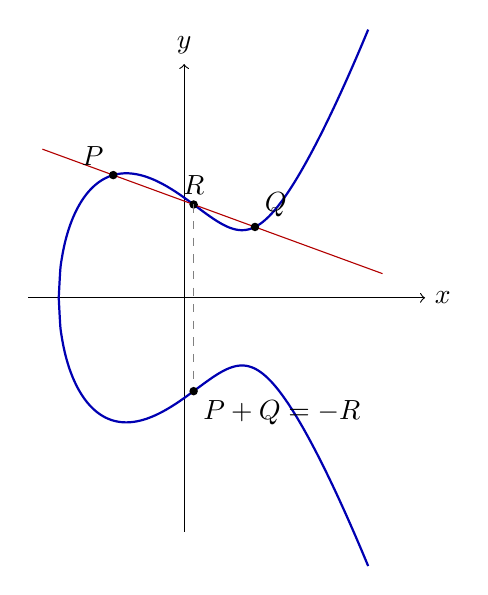
\begin{tikzpicture}[scale=0.9]
  \draw[->] (-2.2,0) -- (3.4,0) node[right] {$x$};
  \draw[->] (0,-3.3) -- (0,3.3) node[above] {$y$};
  % y^2 = x^3 - 2x + 2 approx: draw two branches via plot
  \draw[thick,blue!70!black,domain=-1.7693:2.6,samples=200,smooth] plot (\x,{sqrt(max(\x*\x*\x-2*\x+2,0))});
  \draw[thick,blue!70!black,domain=-1.7693:2.6,samples=200,smooth] plot (\x,{-sqrt(max(\x*\x*\x-2*\x+2,0))});
  % line through P and Q
  \coordinate (P) at (-1,1.732);
  \coordinate (Q) at (1,1);
  \draw[red!70!black] (-2,2.098) -- (2.8,0.341);
  \fill (P) circle (0.06) node[above left] {$P$};
  \fill (Q) circle (0.06) node[above right] {$Q$};
  \fill (0.134,1.317) circle (0.06) node[above] {$R$};
  \draw[dashed,gray] (0.134,1.317) -- (0.134,-1.317);
  \fill (0.134,-1.317) circle (0.06) node[below right] {$P+Q=-R$};
\end{tikzpicture}
\caption{実数点 $y^2=x^3-2x+2$ における弦接法による加法．$P,Q$ を通る直線と曲線の第 3 の交点 $R$ を $x$ 軸で折り返したものが $P+Q$．}
\label{fig:ch17-group-law}
\end{figure}

\paragraph{周期．}
$H_1(E,\Z)=\Z A\oplus\Z B$（$A\cdot B=1$）に対し周期
\[
\omega_1=\int_A\frac{dx}{y},\qquad \omega_2=\int_B\frac{dx}{y},\qquad \tau=\frac{\omega_2}{\omega_1}\in\mathbb{H}
\]
が格子を復元する．これは CY 3-fold の周期 \eqref{eq:ch16-periods}（第16章）の 1 次元版であり，$\tau$ は Weierstrass 形式の係数から周期積分を通して決まる．

\subsection{楕円曲線のモジュライ}

第16章（命題 \ref{prop:ch16-elliptic-iso}，定理 \ref{thm:ch16-j-line}）で見たように，複素楕円曲線の粗モジュライ空間は
\[
\mathcal{M}_{1,1}=\mathbb{H}/\SL(2,\Z)\ \xrightarrow{\ j\ }\ \A^1
\]
である．Weierstrass 形式の言葉で言い直すと，$(g_2,g_3)\in\C^2$ で $\Delta\ne0$ なものと，その上の $\C^*$ 作用 $\lambda\cdot(g_2,g_3)=(\lambda^4g_2,\lambda^6g_3)$（座標変換 $x\mapsto\lambda^2x$, $y\mapsto\lambda^3y$ に対応）による商
\[
\mathcal{M}_{1,1}\cong\{(g_2,g_3)\mid\Delta\ne0\}/\C^*
\]
であり，不変量 $j$ は $\C^*$ 不変な有理関数 $1728g_2^3/\Delta$ に他ならない．
重み $(4,6)$ の重み付き射影直線 $\PP(4,6)$ から $\Delta=0$ の 1 点（cusp，$j=\infty$）を除いたものと見ることもできる．$\Delta=0$ の点を加えた $\PP(4,6)$ は結節 3 次曲線（$I_1$ 型の退化，17.5 節）を加えたコンパクト化 $\overline{\mathcal{M}}_{1,1}$ であり，粗モジュライ空間としては $\PP^1_j$ である．

\begin{myex}{Legendre 標準形}{ch17-legendre}
$y^2=x(x-1)(x-\lambda)$ ($\lambda\ne0,1$) も楕円曲線を与え，
\[
j(\lambda)=256\,\frac{(\lambda^2-\lambda+1)^3}{\lambda^2(\lambda-1)^2}
\]
である．$\lambda$ は 2 等分点の順序付けに依存し，$\lambda\mapsto 1-\lambda,\ 1/\lambda,\dots$ の 6 個の値が同じ $j$ を与える（$\mathfrak{S}_3\cong\SL(2,\Z)/\Gamma(2)$ の作用）．$\lambda$ の空間 $\PP^1\setminus\{0,1,\infty\}$ はレベル 2 構造付きモジュライ $\mathbb{H}/\Gamma(2)$ である．
\end{myex}

\subsection{物理における楕円曲線}

\begin{physbox}[2 次元 CFT とトーラス]
13.6.4 項で見たように，トーラス $T^2=\C/(\Z+\Z\tau)$ 上の 2 次元共形場理論の分配関数 $Z(\tau,\bar\tau)=\Tr_{\mathcal{H}}\,q^{L_0-c/24}\bar q^{\bar L_0-\bar c/24}$ は，$\tau$ と $\gamma\tau$（$\gamma\in\SL(2,\Z)$）が同じトーラスを表すことから\textbf{モジュラー不変}でなければならない．
モジュライの言葉で言えば，$Z$ は $\mathbb{H}$ 上ではなく $\mathcal{M}_{1,1}$ 上の関数である．$T:\tau\to\tau+1$ 不変性はスピン $h-\bar h\in\Z$ を，$S:\tau\to-1/\tau$ 不変性は高温と低温の関係（Cardy 公式による状態数の漸近）を与える．閉弦の 1 ループ振幅は $Z$ を $\mathcal{M}_{1,1}$ の基本領域 $\mathcal{F}$（図 \ref{fig:ch16-fundamental-domain}）上で積分したものであり，$\mathcal{F}$ に紫外領域 $\Img\tau\to0$ が含まれないことが弦理論の紫外有限性の起源である．
\end{physbox}

\begin{physbox}[Seiberg--Witten 曲線]
4 次元 $\mathcal{N}=2$ 超対称 $SU(2)$ ゲージ理論のクーロン相は，ゲージ不変なパラメータ $u=\langle\Tr\phi^2\rangle$ で記述される．Seiberg と Witten は，その低エネルギー有効結合定数
\[
\tau_{\rm eff}(u)=\frac{\theta}{\pi}+\frac{8\pi i}{g^2}
\]
が，$u$ に依存する楕円曲線（ある規格化で）
\[
E_u:\ y^2=(x^2-u)^2-\Lambda^4
\]
のモジュラーパラメータとして与えられることを示した．$\Img\tau_{\rm eff}>0$（結合定数の 2 乗が正）は $\tau\in\mathbb{H}$ と自動的に整合し，電磁双対性 $\SL(2,\Z)$ は $E_u$ の周期の基底の取り替えである．
$u=\pm\Lambda^2$ で $\Delta(E_u)=0$ となり楕円曲線が退化する（サイクルが一つつぶれる）．この点で磁気モノポール（または dyon）が質量ゼロになる．BPS 粒子の質量は周期 $a=\oint_A\lambda$, $a_D=\oint_B\lambda$（$\lambda$ は Seiberg--Witten 微分）で $M=\sqrt2|n_ea+n_ma_D|$ と与えられる．
退化点の周りのモノドロミーは 17.5 節の Kodaira 分類で $I_1$ 型に当たる．
\end{physbox}

\exprob{prob:ch17-1-1}
楕円曲線 $y^2=x^3+fx+g$ について，次のそれぞれの場合に $\Delta=4f^3+27g^2$ と $j$ を計算せよ：(a) $y^2=x^3-x$，(b) $y^2=x^3+1$，(c) $y^2=x^3-3x+2$．ただし (c) では $\Delta=0$ となることを確かめ，曲線の特異点を求め，その特異点が結節点（node）か尖点（cusp）かを判定せよ．

\exprob{prob:ch17-1-2}
Legendre 形 $y^2=x(x-1)(x-\lambda)$ を $x\mapsto x+\frac{1+\lambda}{3}$ と平行移動して $y^2=x^3+fx+g$ の形にし，$f,g$ を $\lambda$ で表せ．これを用いて例 \ref{ex:ch17-legendre} の $j(\lambda)$ の式を確かめよ．

%======================================================================
\section{Mirror symmetry}
%======================================================================

\subsection{Mirror symmetryの基本思想}

第16章で見たように，CY 3-fold $X$ 上の型 IIA 弦理論では K\"ahler モジュライ（$h^{1,1}$ 次元）がベクトル多重項に，複素構造モジュライ（$h^{2,1}$ 次元）がハイパー多重項に入り，型 IIB では逆になる．
ミラー対称性の基本思想は次のとおりである．

\begin{quote}
CY 3-fold $X$ に対し，別の CY 3-fold $\check X$（\textbf{ミラー}）が存在して，$X$ 上の型 IIA 弦理論と $\check X$ 上の型 IIB 弦理論が\textbf{同一の物理}を与える．
\end{quote}

この主張は物理的な双対性であり，そのままの形では数学の定理ではない．数学的にはいくつかの異なる定式化（Hodge 数の対称性，量子コホモロジーと周期の一致，Homological Mirror Symmetry，SYZ 予想）があり，それぞれの状況で証明されているもの，予想にとどまるものがある（17.2.5 項）．

\subsection{Calabi--Yau多様体の双対性}

ミラー対の最も基本的な帰結は Hodge 数の入れ替えである．
\begin{equation}
h^{1,1}(\check X)=h^{2,1}(X),\qquad h^{2,1}(\check X)=h^{1,1}(X),\qquad\text{特に}\ \chi(\check X)=-\chi(X).
\label{eq:ch17-mirror-hodge}
\end{equation}
一般に $h^{p,q}(\check X)=h^{3-p,q}(X)$ であり，CY 3-fold の Hodge ダイアモンドで言えば，\textbf{対角線に関する鏡映}である（図 \ref{fig:ch17-hodge-mirror}）．

\begin{figure}[H]
\centering
\begin{tikzpicture}[scale=0.62]
  \begin{scope}
    \node at (0,3) {$1$};
    \node at (-1,2) {$0$}; \node at (1,2) {$0$};
    \node at (-2,1) {$0$}; \node at (0,1) {$1$}; \node at (2,1) {$0$};
    \node at (-3,0) {$1$}; \node at (-1,0) {$101$}; \node at (1,0) {$101$}; \node at (3,0) {$1$};
    \node at (-2,-1) {$0$}; \node at (0,-1) {$1$}; \node at (2,-1) {$0$};
    \node at (-1,-2) {$0$}; \node at (1,-2) {$0$};
    \node at (0,-3) {$1$};
    \node at (0,-4.3) {quintic $X$};
    \draw[dashed,red!70!black] (-3.5,3.5) -- (3.5,-3.5);
  \end{scope}
  \draw[<->,very thick] (4.3,0) -- node[above] {ミラー} (6.7,0);
  \begin{scope}[xshift=11cm]
    \node at (0,3) {$1$};
    \node at (-1,2) {$0$}; \node at (1,2) {$0$};
    \node at (-2,1) {$0$}; \node at (0,1) {$101$}; \node at (2,1) {$0$};
    \node at (-3,0) {$1$}; \node at (-1,0) {$1$}; \node at (1,0) {$1$}; \node at (3,0) {$1$};
    \node at (-2,-1) {$0$}; \node at (0,-1) {$101$}; \node at (2,-1) {$0$};
    \node at (-1,-2) {$0$}; \node at (1,-2) {$0$};
    \node at (0,-3) {$1$};
    \node at (0,-4.3) {ミラー quintic $\check X$};
  \end{scope}
\end{tikzpicture}
\caption{quintic とそのミラーの Hodge ダイアモンド．$h^{p,q}$ を上から第 $p+q$ 行に並べた（上端 $h^{0,0}$，第 2 行は左から $h^{2,0},h^{1,1},h^{0,2}$，中段は左から $h^{3,0},h^{2,1},h^{1,2},h^{0,3}$）．$h^{p,q}\mapsto h^{3-p,q}$ は破線（左上から右下への対角線）に関する鏡映であり，$h^{1,1}=1$ と $h^{2,1}=101$ が入れ替わる．}
\label{fig:ch17-hodge-mirror}
\end{figure}

\begin{myex}{quintic のミラー（Greene--Plesser）}{ch17-mirror-quintic}
quintic $X$ は $h^{1,1}=1$, $h^{2,1}=101$, $\chi=-200$ である（第15章）．
1 パラメータの族（Dwork 族）
\[
X_\psi:\ x_1^5+x_2^5+x_3^5+x_4^5+x_5^5-5\psi\,x_1x_2x_3x_4x_5=0
\]
を考える．群 $G=\{(\zeta^{a_1},\dots,\zeta^{a_5})\mid\zeta=e^{2\pi i/5},\ \sum a_i\equiv0\}/\Z_5\cong(\Z_5)^3$ は座標の位相変換として $X_\psi$ に作用する．商 $X_\psi/G$ は特異点を持つが，それを crepant に解消（第15章）した $\check X_\psi$ が
\[
h^{1,1}(\check X)=101,\qquad h^{2,1}(\check X)=1,\qquad\chi(\check X)=+200
\]
を持つ CY 3-fold になる．$\check X$ の複素構造モジュライ空間は 1 次元で $\psi^5$ がその座標である．
\end{myex}

\subsection{複素構造とK\"ahler構造の交換}

ミラー対称性は Hodge 数だけでなく，モジュライ空間そのものを交換する：
\[
\mathcal{M}_{\rm K}(X)\ \cong\ \mathcal{M}_{\rm cpx}(\check X)\qquad(\text{局所的に，特殊座標を通じて}),
\]
そして，その上の物理量を一致させる．その代表が 3 点結合（Yukawa 結合）である．
\begin{itemize}
\item \textbf{A 模型}（$X$ 側，K\"ahler モジュライ）：世界面インスタントン（正則曲線）の寄与を含み，
\[
\kappa_{ttt}(t)=\int_XH^3+\sum_{d\ge1}N_d\,d^3\,q^d=5+\sum_{d\ge1}n_d\,d^3\frac{q^d}{1-q^d},\qquad q=e^{2\pi it}.
\]
ここで $N_d$ は次数 $d$ の種数 $0$ Gromov--Witten 不変量，$n_d$ はそこから多重被覆の寄与を除いた整数（\textbf{インスタントン数}，大雑把には次数 $d$ の有理曲線の数）である．A 模型の相関関数は Gromov--Witten 理論で定式化され，複素構造に依存しない．
\item \textbf{B 模型}（$\check X$ 側，複素構造モジュライ）：インスタントン補正を受けず，古典的な周期積分で正確に計算できる：
\[
\kappa_{\psi\psi\psi}=\int_{\check X}\Omega\wedge\partial_\psi^3\Omega .
\]
周期 $\int\Omega$ は Picard--Fuchs 微分方程式（超幾何型）の解であり，具体的に求められる．
\end{itemize}

\begin{mythm}{quintic の種数 0 ミラー定理（Givental, Lian--Liu--Yau）}{ch17-cogp}
ミラー写像（$\check X$ の周期の比で定まる座標変換 $t=t(\psi)$）を通じて B 模型の Yukawa 結合を A 模型の形に書き直したものは，quintic の種数 0 Gromov--Witten 不変量の母関数に一致する．特にインスタントン数は
\[
n_1=2875,\qquad n_2=609250,\qquad n_3=317206375,\ \dots
\]
である．
\end{mythm}

この主張は Candelas--de la Ossa--Green--Parkes（1991）が物理的議論によって\textbf{予言}したものである．$n_1=2875$ は quintic 上の直線の数として 19 世紀から知られていた数（Schubert）であり，$n_2=609250$ は Katz による円錐曲線の数え上げと一致した．任意の次数 $d$ に対する予言は，Givental および Lian--Liu--Yau により数学的に証明された（1996--97）．

\begin{note}
$n_1=2875$ の古典的な導出：$\PP^4$ の直線全体は Grassmann 多様体 $G(2,5)$（6 次元）をなし，5 次式を直線に制限すると $H^0(\PP^1,\OO(5))$（6 次元）の元になる．直線が quintic に含まれる条件は，$G(2,5)$ 上のランク 6 ベクトル束 $\mathrm{Sym}^5S^*$（$S$ は普遍部分束）の切断の零点であり，その個数は Euler 類 $\int_{G(2,5)}c_6(\mathrm{Sym}^5S^*)=2875$ で与えられる．
\end{note}

\subsection{Mirror symmetryの物理的背景}

\begin{physbox}[$\mathcal{N}=(2,2)$ 超共形場理論]
CY 3-fold 上の弦の世界面理論は $c=9$ の $\mathcal{N}=(2,2)$ 超共形場理論（SCFT）である．この理論は左右の $U(1)$ R 対称性を持ち，カイラル環として $(c,c)$ 環と $(a,c)$ 環がある．幾何学的には
\begin{gather*}
(c,c)\ \text{環のチャージ } (1,1) \text{ の元}\ \leftrightarrow\ H^{2,1}(X),\\
(a,c)\ \text{環のチャージ } (-1,1) \text{ の元}\ \leftrightarrow\ H^{1,1}(X)
\end{gather*}

が対応する．一方，左の $U(1)$ チャージの符号を反転する操作は SCFT としては単なる記法の変更であり，これにより $(c,c)$ と $(a,c)$ が入れ替わる．したがって「同じ SCFT を，$H^{1,1}$ と $H^{2,1}$ の役割を入れ替えた二つの CY で実現する」ことが可能であり，それがミラー対である（Lerche--Vafa--Warner, Dixon, Greene--Plesser）．
世界面の位相的ツイストには A ツイストと B ツイストがあり，それぞれ A 模型・B 模型を与える．ミラー対称性は $X$ の A 模型と $\check X$ の B 模型を交換する．
\end{physbox}

物理的な説明としては，ほかに Strominger--Yau--Zaslow（SYZ）による T 双対性の議論がある．$X$ が特殊 Lagrangian 3 次元トーラス $T^3$ によるファイブレーション $X\to B$ を持つとき，各ファイバーで T 双対（$T^3\to\check T^3$）をとったものが $\check X$ である，という主張である（\textbf{SYZ 予想}）．楕円曲線（$T^2=S^1\times S^1$ の一方の $S^1$ で T 双対をとる）では $\tau\leftrightarrow B+i\omega$ の入れ替えとして具体的に確かめられる．

\subsection{数学的発展への概観}

ミラー対称性は，物理から数学への最も成功した「予言」の一つであり，次のような数学的定式化と結果が得られている．
\begin{enumerate}
\item \textbf{位相的ミラー対称性}：Hodge 数の関係 \eqref{eq:ch17-mirror-hodge}．Batyrev はトーリック多様体の反射的多面体の双対性を用いて，トーリック超曲面に対するミラーの組を系統的に構成した（Batyrev--Borisov は完全交差に拡張）．
\item \textbf{閉弦のミラー対称性（種数 0）}：A 模型の量子コホモロジー（Gromov--Witten 不変量）と B 模型の周期（Hodge 構造の変動）が一致する．トーリック完全交差に対しては Givental, Lian--Liu--Yau により定理．高種数（BCOV 理論）は quintic の低い種数で証明が進んでいるが，一般には予想である．
\item \textbf{ホモロジカルミラー対称性}（HMS，Kontsevich 1994）：
\[
D^b(\mathrm{Coh}\,X)\ \simeq\ D^\pi\mathrm{Fuk}(\check X)
\]
（左辺は連接層の導来圏，右辺は Fukaya 圏の導来圏）という三角圏の同値の予想．楕円曲線（Polishchuk--Zaslow），4 次 K3 曲面（Seidel），射影空間内の CY 超曲面（Sheridan ほか）などで証明されているが，一般には\textbf{予想}である．17.4 節で詳しく述べる．
\item \textbf{SYZ 予想}：特殊 Lagrangian トーラスファイブレーションの存在とその双対としてのミラー．特異ファイバーの扱いが難しく一般には未解決であり，Gross--Siebert プログラムなどの代数的な定式化が進んでいる．
\end{enumerate}

\exprob{prob:ch17-2-1}
CY 3-fold の Euler 数が $\chi=2(h^{1,1}-h^{2,1})$ で与えられることを，Hodge ダイアモンド（$h^{p,0}=0$ ($p=1,2$), $h^{3,0}=1$）と $\chi=\sum_{p,q}(-1)^{p+q}h^{p,q}$ から示せ．これを用いて quintic とそのミラーの Euler 数を求めよ．

\exprob{prob:ch17-2-2}
A 模型の Yukawa 結合 $\kappa_{ttt}=5+\sum_{d\ge1}n_dd^3\frac{q^d}{1-q^d}$ を $q$ について展開し，$q^1$, $q^2$ の係数を $n_1,n_2$ で表せ．さらに $n_1=2875$, $n_2=609250$ を代入して，$q^2$ の係数に「直線の 2 重被覆」からの寄与がどれだけ含まれるか答えよ．

%======================================================================
\section{幾何学的遷移}
%======================================================================

\subsection{特異点を介した幾何学的変化}

CY 3-fold のモジュライ空間には境界があり，そこでは $X$ が特異になる．
複素構造モジュライの境界では「3 次元球面 $S^3$ がつぶれ」，K\"ahler モジュライの境界（K\"ahler 錐の壁．図 \ref{fig:ch16-kahler-cone}）では「2 次元球面 $S^2$ がつぶれる」．
同じ特異 CY が両方の極限として現れるとき，特異点を通過して\textbf{位相の異なる}CY 3-fold へ移ることができる．これを\textbf{幾何学的遷移}という．

\begin{mydef}{幾何学的遷移}{ch17-geometric-transition}
滑らかな CY 3-fold $X$, $Y$ と特異 CY 3-fold $X_0$ があり，
(i) $X_0$ は $X$ の複素構造の退化（$X$ の族の特殊ファイバー）として得られ，
(ii) $Y\to X_0$ は crepant な特異点解消（$K_Y=\pi^*K_{X_0}$）である
とき，$X\rightsquigarrow X_0\leftarrow Y$ を\textbf{幾何学的遷移}という．
\end{mydef}

\subsection{Blow-upとBlow-down}

第15章で見たように，blow-up は点や部分多様体を例外因子で置き換える操作であり，blow-down はその逆である．
CY を保つ（$c_1=0$ を保つ）ためには解消が crepant でなければならないが，3-fold の孤立点の通常の blow-up は一般に crepant でない．
例えば $\C^3$ の原点の blow-up では例外因子 $E\cong\PP^2$ が現れ $K=\pi^*K+2E$ となり CY 条件が壊れる．
そこで次の\textbf{小解消}（small resolution）が重要になる：例外集合が因子ではなく曲線（余次元 2）であるような解消．このとき $K$ の変化を担う因子がないので自動的に crepant である．

\subsection{Calabi--Yauの幾何学的遷移}

CY 3-fold の最も基本的な特異点は\textbf{結節点}（node，ordinary double point，conifold 特異点）である（第15章）．局所的には
\begin{equation}
X_0:\ z_1^2+z_2^2+z_3^2+z_4^2=0\ \subset\C^4
\label{eq:ch17-conifold}
\end{equation}
で与えられる．これは原点を頂点とする錐であり，底（$|z|=1$ との交わり）は $S^2\times S^3$ と同相である．

\paragraph{変形（deformation）．}
方程式を
\[
X_\varepsilon:\ z_1^2+z_2^2+z_3^2+z_4^2=\varepsilon\qquad(\varepsilon>0)
\]
と変形すると滑らかになる．$z_k=x_k+iy_k$ と書けば $|x|^2-|y|^2=\varepsilon$, $x\cdot y=0$ であり，$y=0$ の部分は半径 $\sqrt\varepsilon$ の $S^3$ である．実際 $X_\varepsilon\cong T^*S^3$（$S^3$ の余接束）であり，$\varepsilon\to0$ で\textbf{特殊 Lagrangian な $S^3$（消滅サイクル）がつぶれる}．

\paragraph{小解消（small resolution）．}
座標変換 $x=z_1+iz_2$, $y=z_1-iz_2$, $z=z_3+iz_4$, $w=-z_3+iz_4$ を行うと $xy-zw=\sum_kz_k^2$ なので，\eqref{eq:ch17-conifold} は
\[
X_0:\ xy-zw=0\qquad\Longleftrightarrow\qquad \rank\begin{pmatrix}x&z\\w&y\end{pmatrix}\le1
\]
と書ける．
\[
Y=\Bigl\{\bigl((x,y,z,w),(\lambda:\mu)\bigr)\in\C^4\times\PP^1\ \Big|\ \begin{pmatrix}x&z\\w&y\end{pmatrix}\begin{pmatrix}\lambda\\-\mu\end{pmatrix}=0\Bigr\}
\]
とおくと，射影 $Y\to X_0$ は原点以外で同型，原点の逆像は $\PP^1\cong S^2$ である．$Y$ は $\PP^1$ 上のベクトル束 $\OO(-1)\oplus\OO(-1)$ の全空間と同型であり，例外集合 $\PP^1$ は曲線なので小解消（crepant）である．行列の左側から掛ける条件 $(\lambda',\mu')\bigl(\begin{smallmatrix}x&z\\w&y\end{smallmatrix}\bigr)=0$ で定める別の小解消 $Y'$ もあり，$Y$ と $Y'$ は \textbf{flop} で移り合う．

\subsection{Conifold transition}

\begin{figure}[H]
\centering
\begin{tikzpicture}[scale=0.85]
  % deformed: cone with S^3 neck
  \begin{scope}
    \draw[thick] (-1.6,2) .. controls (-0.5,0.7) and (-0.5,-0.7) .. (-1.6,-2);
    \draw[thick] (1.6,2) .. controls (0.5,0.7) and (0.5,-0.7) .. (1.6,-2);
    \draw[thick] (0,2) ellipse (1.6 and 0.3);
    \draw[thick,red!70!black] (0,0) ellipse (0.47 and 0.12);
    \node[red!70!black] at (0,-0.5) {$S^3$};
    \node at (0,-2.7) {変形 $X_\varepsilon$};
    \node at (0,-3.25) {\small $\sum z_i^2=\varepsilon$};
  \end{scope}
  \draw[->,thick] (2.0,0) -- node[above] {\small $\varepsilon\to0$} (3.4,0);
  % singular
  \begin{scope}[xshift=5.2cm]
    \draw[thick] (-1.6,2) -- (0,0) -- (-1.6,-2);
    \draw[thick] (1.6,2) -- (0,0) -- (1.6,-2);
    \draw[thick] (0,2) ellipse (1.6 and 0.3);
    \fill (0,0) circle (0.07);
    \node at (0,-2.7) {conifold $X_0$};
    \node at (0,-3.25) {\small $\sum z_i^2=0$};
  \end{scope}
  \draw[<-,thick] (7.0,0) -- node[above] {\small 小解消} (8.4,0);
  % resolved
  \begin{scope}[xshift=10.4cm]
    \draw[thick] (-1.6,2) .. controls (-0.6,0.8) .. (-0.55,0.25);
    \draw[thick] (-0.55,-0.25) .. controls (-0.6,-0.8) .. (-1.6,-2);
    \draw[thick] (1.6,2) .. controls (0.6,0.8) .. (0.55,0.25);
    \draw[thick] (0.55,-0.25) .. controls (0.6,-0.8) .. (1.6,-2);
    \draw[thick] (0,2) ellipse (1.6 and 0.3);
    \draw[thick,blue!70!black,fill=blue!10] (0,0) circle (0.55);
    \draw[blue!70!black] (0,0) ellipse (0.55 and 0.15);
    \node[blue!70!black] at (1.15,-0.1) {$S^2$};
    \node at (0,-2.7) {小解消 $Y$};
    \node at (0,-3.25) {\small $\OO(-1)\oplus\OO(-1)\to\PP^1$};
  \end{scope}
\end{tikzpicture}
\caption{conifold transition の模式図．左：複素構造の変形で $S^3$ が現れる（$T^*S^3$）．中：$S^3$（または $S^2$）がつぶれた conifold 特異点．右：小解消で頂点が $S^2=\PP^1$ に置き換わる．いずれも無限遠では錐 $S^2\times S^3$ に漸近する．}
\label{fig:ch17-conifold-transition}
\end{figure}

コンパクトな CY では，結節点はいくつかまとめて現れる．
$X$ が $N$ 個の結節点を持つ $X_0$ に退化し，$N$ 個の消滅 $S^3$ の間に $H_3(X)$ で $r$ 個の独立な線形関係があるとする．小解消 $Y$ が（射影的な）CY になるとき，
\begin{equation}
h^{1,1}(Y)=h^{1,1}(X)+r,\qquad h^{2,1}(Y)=h^{2,1}(X)-N+r,\qquad \chi(Y)=\chi(X)+2N
\label{eq:ch17-transition-hodge}
\end{equation}
が成り立つ（Euler 数は，$\chi=0$ の $S^3$ を $\chi=2$ の $S^2$ で $N$ 回置き換えることから）．

\begin{myex}{16 個の結節点を持つ quintic}{ch17-quintic-transition}
$\PP^4$ の quintic を特殊化して
\[
X_0:\ x_1\,g(x)+x_2\,h(x)=0\qquad(g,h\ \text{は一般の 4 次式})
\]
とする．これは平面 $\{x_1=x_2=0\}\cong\PP^2$ を含み，$x_1=x_2=g=h=0$ の $4\times4=16$ 点で結節点を持つ．
\[
Y=\{\,(x,(\lambda:\mu))\in\PP^4\times\PP^1\mid \lambda x_1+\mu x_2=0,\ \mu g(x)-\lambda h(x)=0\,\}
\]
は $X_0$ の小解消であり，$r=1$ なので \eqref{eq:ch17-transition-hodge} より
\[
(h^{1,1},h^{2,1})=(1,101)\ \rightsquigarrow\ (2,\,101-16+1)=(2,86),\qquad \chi:\ -200\to-168 .
\]
\end{myex}

\subsection{物理的解釈}

\begin{physbox}[Strominger の質量ゼロ黒穴と相転移]
conifold 点の近くでは，消滅サイクル $A$ の周期 $z=\int_A\Omega\to0$ に対し，双対サイクル $B$ の周期が
\[
\int_B\Omega\ \simeq\ \frac{z}{2\pi i}\log z+(\text{正則})
\]
と振る舞う（Picard--Lefschetz 公式：$z$ の周りを一周すると $B\to B+A$）．このため Weil--Petersson 計量は $G_{z\bar z}\sim-\log|z|^2$ と発散し，古典的な有効理論は conifold 点で特異になる．

Strominger（1995）は，型 IIB 理論で D3 ブレーンが消滅 $S^3$ に巻き付いた状態を考えた．その質量は $M\propto|\int_{S^3}\Omega|=|z|$ であり，conifold 点で\textbf{質量ゼロ}になる．4 次元ではこれは電荷を持つ極限的黒穴（BPS 状態）である．この粒子を有効理論から積分すると，ちょうど 1 ループで $\log|z|$ の特異性が再現される．すなわち特異性は「軽くなった粒子を積分してしまった」ことの帰結であり，それを有効理論に含めれば理論は滑らかである．

さらに Greene--Morrison--Strominger は，$N$ 個の結節点がある場合に質量ゼロのハイパー多重項 $N$ 個が $N-r$ 個の $U(1)$ ベクトル多重項に電荷を持ち，それらが凝縮（Higgs 相に移行）すると $N-r$ 個のベクトル多重項が質量を得て $r$ 個の中性ハイパー多重項が残ることを示した．IIB では（第16章の表）ベクトル多重項数 $=h^{2,1}$，ハイパー多重項数 $=h^{1,1}+1$ なので，これはちょうど \eqref{eq:ch17-transition-hodge} の Hodge 数の変化である．位相の異なる CY が，物理的には\textbf{一つのモジュライ空間の異なる相}として滑らかにつながっている．
\end{physbox}

\exprob{prob:ch17-3-1}
\eqref{eq:ch17-transition-hodge} を用いて，例 \ref{ex:ch17-quintic-transition} の $Y$ の Euler 数を Hodge 数から計算し，$\chi(X)+2N$ と一致することを確かめよ．また IIB 理論のベクトル多重項とハイパー多重項の数が遷移の前後でどう変わるか答えよ．

\exprob{prob:ch17-3-2}
$X_\varepsilon:\sum_{k=1}^4z_k^2=\varepsilon$（$\varepsilon>0$）において，$z_k=x_k+iy_k$ とおき，$X_\varepsilon$ が $\{(x,y)\in\R^4\times\R^4\mid |x|^2=\varepsilon+|y|^2,\ x\cdot y=0\}$ と書けることを示せ．これを用いて $X_\varepsilon$ が $S^3$ の接束（$\cong$ 余接束）と微分同相であることを説明せよ．

%======================================================================
\section{D-braneと幾何学}
%======================================================================

\subsection{D-braneの幾何学的背景}

開弦は端点を持ち，その端点の境界条件として Dirichlet 条件が課される部分多様体を \textbf{D ブレーン}という（Polchinski 1995）．D ブレーンは R-R 場の電荷を持つ動的な物体であり，その上には開弦の質量ゼロのモードとしてゲージ場が住む．
内部空間 $X$ が CY のとき，4 次元で超対称性を保つ（BPS な）D ブレーンは，$X$ の\textbf{幾何学的に特別な}部分多様体に巻き付いたものでなければならない．世界面の超対称性の境界条件には 2 種類あり，それに応じて
\begin{itemize}
\item \textbf{B 型ブレーン}（B-brane）：複素部分多様体に巻き付き，複素構造にのみ依存する（K\"ahler 構造には安定性条件を通じてのみ依存）．
\item \textbf{A 型ブレーン}（A-brane）：特殊 Lagrangian 部分多様体に巻き付き，シンプレクティック構造（K\"ahler 形式 $\omega$）に依存する．
\end{itemize}
の 2 種類が現れる．

\subsection{Braneと部分多様体}

\begin{mydef}{特殊 Lagrangian 部分多様体}{ch17-slag}
CY $n$-fold $(X,\omega,\Omega)$ の実 $n$ 次元部分多様体 $L$ が \textbf{Lagrangian} とは $\omega|_L=0$ であることをいい，さらに $\Img(e^{-i\theta}\Omega)|_L=0$（ある定数 $\theta$）を満たすとき\textbf{位相 $\theta$ の特殊 Lagrangian} という．このとき $\Re(e^{-i\theta}\Omega)|_L$ は $L$ の体積形式であり，$L$ はそのホモロジー類の中で体積最小（キャリブレーション）である．
\end{mydef}

例えば conifold の変形 $X_\varepsilon$ の $S^3=\{y=0\}$ は特殊 Lagrangian であり，17.3 節の D3 ブレーンはこれに巻き付いている．
一方，B 型ブレーンの台は複素部分多様体（点，正則曲線，因子，$X$ 全体）であり，これらも K\"ahler 形式によるキャリブレーション（Wirtinger の不等式）で体積最小である．

\subsection{Brane上の束}

D ブレーンの世界体積上にはゲージ場 $A$ が住むので，ブレーンのデータは「部分多様体 $Z$」と「$Z$ 上のベクトル束 $E$ と接続」の組である．$N$ 枚のブレーンが重なると $U(N)$ ゲージ理論になり，$E$ はランク $N$ の束となる（第14章）．
超対称性の条件は
\begin{itemize}
\item B 型：$Z$ は複素部分多様体，$E$ は\textbf{正則}ベクトル束（曲率が $(1,1)$ 型：$F^{0,2}=0$）で，さらに Hermite--Yang--Mills 方程式（安定性に対応）を満たす．
\item A 型：$L$ は特殊 Lagrangian，$E$ は\textbf{平坦}な $U(N)$ 束（$F=0$）．
\end{itemize}
したがって B 型ブレーンは代数幾何学の対象 $(Z,E)$ で記述される．これを $X$ 上の層として見たのが次の考え方である．

\subsection{Braneと代数的構造}

複素部分多様体 $i:Z\hookrightarrow X$ 上の正則ベクトル束 $E$ に対し，押し出し $i_*E$ は $X$ 上の\textbf{連接層}である（層については第11章）．
例えば型 IIA 理論で点 $p$ に局在した D0 ブレーンは摩天楼層 $\OO_p$ に，$X$ 全体に巻き付いた 1 枚の D6 ブレーンは構造層 $\OO_X$ に，正則曲線 $C$ に巻き付いた D2 ブレーンは $i_*\OO_C$（あるいは $C$ 上の直線束の押し出し）に対応する．
こうして
\[
\text{B 型ブレーン}\ \longleftrightarrow\ X\ \text{上の連接層}\ \sheaf{F}
\]
という対応が得られる．D ブレーンの電荷（R-R 電荷）は層の Chern 指標から
\[
Q(\sheaf{F})=\mathrm{ch}(\sheaf{F})\sqrt{\mathrm{Td}(X)}\in H^{\rm even}(X,\Q)
\]
（Minasian--Moore）で与えられ，より正確には K 理論の類である．

二つのブレーン $\sheaf{E},\sheaf{F}$ の間に張られる開弦の質量ゼロ状態は
\[
\mathrm{Ext}^k_X(\sheaf{E},\sheaf{F})\qquad(k=0,1,2,3)
\]
で与えられ，$k$ は開弦の状態の $U(1)$ R チャージ（ghost number）に当たる．$\sheaf{E}=\sheaf{F}=\OO_Z$ のときの $\mathrm{Ext}^1$ はブレーンの変形（モジュライ）であり，これは第16章の変形理論のブレーン版である．

\subsection{Derived categoryへの導入}

連接層だけではすべての B 型ブレーンを記述できない．ブレーンと反ブレーンの系では，その間の開弦にタキオンが現れ，タキオン凝縮によって新しいブレーンが生じる．これを数学的に捉えるには，層そのものではなく層の\textbf{複体}を考える必要がある（Douglas, Sharpe, Aspinwall--Lawrence）．

\begin{mydef}{連接層の導来圏（概略）}{ch17-derived-category}
$X$ 上の連接層の有界な複体
\[
\sheaf{E}^\bullet:\ \cdots\to\sheaf{E}^{k-1}\xrightarrow{d}\sheaf{E}^{k}\xrightarrow{d}\sheaf{E}^{k+1}\to\cdots\qquad(d^2=0,\ \text{有限個を除いて } 0)
\]
を対象とし，複体の射のうちコホモロジー層の同型を誘導するもの（\textbf{擬同型}）を形式的に可逆にして得られる圏を\textbf{有界導来圏} $D^b(\mathrm{Coh}\,X)$ という．
シフト $\sheaf{E}^\bullet[n]$（$\sheaf{E}[n]^k=\sheaf{E}^{n+k}$）があり，
\[
\Hom_{D^b(X)}(\sheaf{E},\sheaf{F}[k])=\mathrm{Ext}^k(\sheaf{E},\sheaf{F})
\]
が成り立つ．$D^b(\mathrm{Coh}\,X)$ は加法圏ではあるが Abel 圏ではなく，\textbf{三角圏}の構造（完全三角 $\sheaf{E}\to\sheaf{F}\to\sheaf{G}\to\sheaf{E}[1]$）を持つ．
\end{mydef}

物理的には，
\begin{itemize}
\item 複体 $\sheaf{E}\xrightarrow{T}\sheaf{F}$（$\sheaf{E}$ を奇数次に置く）は，ブレーン $\sheaf{F}$ と反ブレーン $\sheaf{E}$ の間にタキオン $T$ が凝縮した状態，
\item 擬同型による同一視は，くりこみ群の流れで同じ IR の状態に流れることの表現，
\item シフト $[1]$ はブレーンを反ブレーンに変える操作，
\end{itemize}
と解釈される．

\begin{myex}{$\PP^1$ 上の Ext}{ch17-ext-p1}
$\mathrm{Ext}^k_{\PP^1}(\OO(a),\OO(b))=H^k(\PP^1,\OO(b-a))$ であり，
$\dim\mathrm{Ext}^0=\max(b-a+1,0)$，$\dim\mathrm{Ext}^1=\max(a-b-1,0)$．
例えば $\mathrm{Ext}^1(\OO,\OO(-2))\cong H^1(\PP^1,\OO(-2))\cong\C$ であり，対応する非自明な拡大は Euler 列 $0\to\OO(-2)\to\OO(-1)^{\oplus2}\to\OO\to0$ である．完全三角 $\OO(-2)\to\OO(-1)^{\oplus2}\to\OO\to\OO(-2)[1]$ は「$\OO(-1)^{\oplus2}$ は $\OO$ と $\OO(-2)$ の束縛状態である」と読める．
\end{myex}

\begin{physbox}[Homological Mirror Symmetry と安定性]
A 型ブレーン（特殊 Lagrangian ＋平坦束）とその間の開弦（Floer コホモロジー）は \textbf{Fukaya 圏} $\mathrm{Fuk}(\check X)$ をなす．Kontsevich の \textbf{Homological Mirror Symmetry 予想}は
\[
D^b(\mathrm{Coh}\,X)\ \simeq\ D^\pi\mathrm{Fuk}(\check X)
\]
という三角圏の同値を主張する（B 型ブレーン on $X$ ＝ A 型ブレーン on $\check X$）．これは前節で述べたとおり，いくつかの場合に証明された\textbf{予想}である．
楕円曲線では，$\OO_p$（点）が $\check E$ 上の「縦の」円周に，$\OO_E$ が「横の」円周に移り，$\Hom(\OO_E,\OO_p)\cong\C$（Serre 双対で $\mathrm{Ext}^1(\OO_p,\OO_E)\cong\C$）が二つの円周のただ一つの交点に対応する．
導来圏のすべての対象が物理的に安定な BPS ブレーンになるわけではなく，どれが安定かは K\"ahler モジュライ（B 型の場合）に依存する．これを定式化したのが Douglas の $\Pi$ 安定性と，それを数学的に整備した Bridgeland の\textbf{安定性条件}である．
\end{physbox}

\exprob{prob:ch17-4-1}
$\PP^1$ 上で $\mathrm{Ext}^k(\OO(a),\OO(b))$ を $k=0,1$ について計算し，Serre 双対性 $\mathrm{Ext}^k(\sheaf{E},\sheaf{F})\cong\mathrm{Ext}^{1-k}(\sheaf{F},\sheaf{E}\otimes K_{\PP^1})^*$（$K_{\PP^1}=\OO(-2)$）と整合することを確かめよ．

\exprob{prob:ch17-4-2}
CY 3-fold $X$ 上の連接層 $\sheaf{E},\sheaf{F}$ について，Serre 双対性 $\mathrm{Ext}^k(\sheaf{E},\sheaf{F})\cong\mathrm{Ext}^{3-k}(\sheaf{F},\sheaf{E}\otimes K_X)^*$ と $K_X\cong\OO_X$ から，$\mathrm{Ext}^k(\sheaf{E},\sheaf{F})\cong\mathrm{Ext}^{3-k}(\sheaf{F},\sheaf{E})^*$ を導け．$\sheaf{E}=\sheaf{F}$ のとき $\mathrm{Ext}^1$ と $\mathrm{Ext}^2$（ブレーンのモジュライと障害）の次元が等しいことの物理的意味を，「モジュライ場とその超ポテンシャル」の言葉で説明せよ．

%======================================================================
\section{F-theoryへの接続}
%======================================================================

\subsection{F-theoryの幾何学的背景}

型 IIB 超弦理論には二つのスカラー場，R-R の axion $C_0$ とディラトン $\phi$ があり，これを組み合わせた
\begin{equation}
\tau=C_0+i\,e^{-\phi}\in\mathbb{H}
\label{eq:ch17-axio-dilaton}
\end{equation}
を\textbf{軸・ディラトン}（axio-dilaton）という．$\Img\tau=1/g_s>0$ である．IIB 理論は $\SL(2,\Z)$ 双対性
\[
\tau\mapsto\frac{a\tau+b}{c\tau+d}
\]
を持つと信じられており（$S$ は強弱双対 $g_s\to1/g_s$），物理的に区別される $\tau$ の値は $\mathbb{H}/\SL(2,\Z)=\mathcal{M}_{1,1}$ にある．これは楕円曲線のモジュライ空間そのものである．

Vafa（1996）の着想は，\textbf{$\tau$ を補助的な楕円曲線（トーラス）のモジュラーパラメータとみなし}，時空の各点にその楕円曲線を付け加えることである．IIB 理論が 10 次元時空 $\R^{1,3}\times B$（$B$ は実 6 次元の内部空間）上にあり $\tau$ が $B$ 上で変化するとき，$B$ の各点 $b$ に楕円曲線 $E_{\tau(b)}$ を付けた 12 次元の空間（形式的な）が得られる．これが \textbf{F 理論}の幾何学である．楕円ファイバーの大きさは物理的な意味を持たず，複素構造 $\tau$ だけが意味を持つ．

\subsection{楕円ファイバー}

\begin{mydef}{楕円ファイブレーション}{ch17-elliptic-fibration}
射影多様体 $Y$ から $B$ への全射 $\pi:Y\to B$ が\textbf{楕円ファイブレーション}であるとは，一般のファイバー $\pi^{-1}(b)$ が滑らかな楕円曲線（種数 $1$ の曲線）であることをいう．さらに切断 $\sigma:B\to Y$（$\pi\circ\sigma=\mathrm{id}$）があるとき，各ファイバーは原点 $\sigma(b)$ を持つ楕円曲線になる．
\end{mydef}

ファイバーの $\tau(b)$ は $B$ 上で正則に変化する（$j(\tau(b))$ が $B$ 上の有理関数）．ファイバーが特異になる点の集合を\textbf{判別式軌跡} $\Delta\subset B$ という．$\Delta$ の周りを一周すると，ファイバーの $H_1$ の基底が $\SL(2,\Z)$ の元（\textbf{モノドロミー}）で変換され，それに伴い $\tau$ が $\SL(2,\Z)$ 変換を受ける．
IIB の言葉では，この $\SL(2,\Z)$ モノドロミーは 7 ブレーンの存在を意味する．例えば $\tau\to\tau+1$ のモノドロミーは $\oint dC_0=1$，すなわち D7 ブレーン 1 枚の R-R 電荷である．

\subsection{Elliptic fibration}

\begin{figure}[H]
\centering
\begin{tikzpicture}[scale=0.9]
  % base
  \draw[thick] (-0.5,0) -- (11,0) node[right] {$B$};
  % generic tori
  \foreach \x in {0.8,3.2,7.2,10}{
    \draw[thick,blue!70!black] (\x,2.2) ellipse (0.55 and 0.95);
    \draw[blue!70!black] (\x-0.12,2.55) arc (120:240:0.38);
    \draw[blue!70!black] (\x-0.2,2.45) arc (60:-60:0.26);
    \draw[gray,dashed] (\x,0) -- (\x,1.2);
    \fill (\x,0) circle (0.04);
  }
  % I1 pinched fiber
  \begin{scope}[xshift=5.2cm]
    \draw[thick,red!70!black] (0,3.15) .. controls (0.8,3.0) and (0.6,1.6) .. (0,2.2)
      .. controls (-0.6,1.6) and (-0.8,3.0) .. (0,3.15);
    \draw[thick,red!70!black] (0,2.2) .. controls (0.5,1.4) and (0.4,1.2) .. (0,1.25)
      .. controls (-0.4,1.2) and (-0.5,1.4) .. (0,2.2);
    \fill[red!70!black] (0,2.2) circle (0.06);
    \draw[gray,dashed] (0,0) -- (0,1.2);
    \fill[red!70!black] (0,0) circle (0.07);
    \node[below,red!70!black] at (0,-0.1) {$\Delta=0$};
    \node[red!70!black,anchor=west] at (0.55,1.05) {\small 特異ファイバー};
    \node[red!70!black,anchor=west] at (0.55,0.7) {\small （7 ブレーン）};
  \end{scope}
  \node[blue!70!black] at (2.0,3.6) {\small 滑らかな $E_{\tau(b)}$};
  \draw[->] (5.6,-0.9) arc (-30:210:0.45 and 0.25);
  \node at (7.1,-0.9) {\small モノドロミー $\in\SL(2,\Z)$};
\end{tikzpicture}
\caption{楕円ファイブレーション $\pi:Y\to B$ の模式図．一般のファイバーは楕円曲線 $E_{\tau(b)}$ で，判別式 $\Delta=0$ の上でファイバーが退化する（図は 1 つのサイクルがつぶれた $I_1$ 型）．F 理論ではそこに 7 ブレーンがあり，周りを回ると $\tau$ が $\SL(2,\Z)$ 変換を受ける．}
\label{fig:ch17-elliptic-fibration}
\end{figure}

F 理論が超対称性を保つための条件は，全空間 $Y$ が \textbf{Calabi--Yau} であることである．$B$ を複素 $n-1$ 次元とすると，
\begin{itemize}
\item F 理論 on 楕円 K3 $\to\PP^1$：8 次元の理論（$n=2$），
\item F 理論 on 楕円 CY 3-fold $\to B_2$：6 次元の理論（$n=3$），
\item F 理論 on 楕円 CY 4-fold $\to B_3$：4 次元 $\mathcal{N}=1$ の理論（$n=4$）．
\end{itemize}
基底 $B$ 自体は CY ではない（$\tau$ の変化，すなわち 7 ブレーンのエネルギーが $B$ を曲げる）．

\subsection{Weierstrass model}

切断を持つ楕円ファイブレーションは（双有理的に）\textbf{Weierstrass モデル}
\begin{equation}
Y:\ y^2=x^3+f\,x+g,\qquad f\in H^0(B,\mathcal{L}^{4}),\ g\in H^0(B,\mathcal{L}^{6})
\label{eq:ch17-weierstrass-model}
\end{equation}
で書ける．ここで $\mathcal{L}$ は $B$ 上の直線束で，$x,y$ はそれぞれ $\mathcal{L}^2,\mathcal{L}^3$ の切断として扱う（楕円曲線の $\C^*$ 作用の重み $(4,6)$ と同じ構造：17.1.4 項）．判別式は
\[
\Delta=4f^3+27g^2\in H^0(B,\mathcal{L}^{12}),\qquad j=1728\,\frac{4f^3}{\Delta}
\]
である．

\begin{myprop}{Calabi--Yau 条件}{ch17-cy-condition}
Weierstrass モデル \eqref{eq:ch17-weierstrass-model} の全空間が（特異点を除いて）$K_Y\cong\OO_Y$ を満たすための条件は $\mathcal{L}=K_B^{-1}$ である．すなわち
\[
f\in H^0(B,K_B^{-4}),\qquad g\in H^0(B,K_B^{-6}),\qquad \Delta\in H^0(B,K_B^{-12}).
\]
\end{myprop}

\begin{proof}[証明の概略]
随伴公式により $K_Y=\pi^*(K_B\otimes\mathcal{L})$ となる（ファイバー方向の正則 1 形式 $dx/y$ は $\mathcal{L}^{-1}$ の重みを持つ）．$K_Y$ が自明になるのは $K_B\otimes\mathcal{L}\cong\OO_B$ のときである．
\end{proof}

\begin{myex}{楕円 K3 と 24 枚の 7 ブレーン}{ch17-elliptic-k3}
$B=\PP^1$ では $K_B^{-1}=\OO(2)$ なので，$f,g,\Delta$ はそれぞれ次数 $8,12,24$ の多項式である．一般には $\Delta$ は 24 個の単純零点を持ち，そこに 24 枚の 7 ブレーンがある．
楕円 K3 の Euler 数は $\chi(K3)=24$ であり，これは「一般ファイバー（$\chi=0$）」と「24 個の $I_1$ 型ファイバー（各 $\chi=1$）」から $\chi=24\times1$ として再現される．
F 理論 on 楕円 K3 は，ヘテロティック弦 on $T^2$ と双対である（8 次元）．
\end{myex}

\subsection{特異ファイバーとゲージ群}

判別式 $\Delta$ の既約成分 $\{w=0\}\subset B$ に沿ったファイバーの退化の型は，$f,g,\Delta$ の $w$ に関する零点の位数 $(\mathrm{ord}\,f,\mathrm{ord}\,g,\mathrm{ord}\,\Delta)$ で決まる．これが \textbf{Kodaira の分類}（楕円曲面の特異ファイバーの分類，Tate のアルゴリズム）である．
特異ファイバーを解消すると，ファイバーは $\PP^1$ の木（または輪）になり，その交差のグラフは（affine）Dynkin 図形になる．F 理論ではこの Dynkin 図形の Lie 代数が 7 ブレーン上の\textbf{ゲージ代数}を与える．

\begin{table}[H]
\centering
\small
\setlength{\tabcolsep}{4pt}
\renewcommand{\arraystretch}{1.25}
\begin{tabular}{cccccc}
\hline
型 & $\mathrm{ord}\,f$ & $\mathrm{ord}\,g$ & $\mathrm{ord}\,\Delta$ & 解消したファイバー & ゲージ代数\\
\hline
$I_0$ & $\ge0$ & $\ge0$ & $0$ & 滑らかな楕円曲線 & なし\\
$I_n$ ($n\ge1$) & $0$ & $0$ & $n$ & $\PP^1$ $n$ 個の輪 $\tilde A_{n-1}$ & $\mathfrak{su}(n)$\\
$II$ & $\ge1$ & $1$ & $2$ & 尖点曲線 & なし\\
$III$ & $1$ & $\ge2$ & $3$ & 接する $\PP^1$ 2 個 $\tilde A_1$ & $\mathfrak{su}(2)$\\
$IV$ & $\ge2$ & $2$ & $4$ & 1 点で交わる $\PP^1$ 3 個 $\tilde A_2$ & $\mathfrak{su}(3)$\\
$I_0^*$ & $\ge2$ & $\ge3$ & $6$ & $\tilde D_4$ & $\mathfrak{so}(8)$\\
$I_n^*$ ($n\ge1$) & $2$ & $3$ & $n+6$ & $\tilde D_{n+4}$ & $\mathfrak{so}(2n+8)$\\
$IV^*$ & $\ge3$ & $4$ & $8$ & $\tilde E_6$ & $\mathfrak{e}_6$\\
$III^*$ & $3$ & $\ge5$ & $9$ & $\tilde E_7$ & $\mathfrak{e}_7$\\
$II^*$ & $\ge4$ & $5$ & $10$ & $\tilde E_8$ & $\mathfrak{e}_8$\\
\hline
（非極小） & $\ge4$ & $\ge6$ & $\ge12$ & \multicolumn{2}{l}{CY を保つ解消なし（$B$ の blow-up が必要）}\\
\hline
\end{tabular}
\caption{Kodaira の分類と F 理論のゲージ代数．$I_1$ は結節点，$II$ は尖点を持つ既約な特異 3 次曲線．ゲージ代数は，ファイバーの成分が判別式成分の周りのモノドロミーで入れ替わらない（split）場合のもの．入れ替わる場合（non-split）は折り返した代数になる（例：$I_n\to\mathfrak{sp}(\lfloor n/2\rfloor)$，$IV\to\mathfrak{sp}(1)$，$I_0^*\to\mathfrak{g}_2$ または $\mathfrak{so}(7)$，$IV^*\to\mathfrak{f}_4$）．}
\label{tab:ch17-kodaira}
\end{table}

\begin{myex}{$n$ 枚の D7 ブレーンと $SU(n)$}{ch17-In}
$\Delta$ が $w=0$ で単純零点を持ち $f,g$ が消えないとき（$I_1$），$w$ の周りのモノドロミーは $T=\bigl(\begin{smallmatrix}1&1\\0&1\end{smallmatrix}\bigr)$ であり，ここに 1 枚の D7 ブレーンがある．$n$ 枚が重なる（$I_n$, $\mathrm{ord}\,\Delta=n$）とモノドロミーは $T^n$ となり，D7 ブレーンの積み重ねの上の $U(n)$ のうち $SU(n)$ 部分がゲージ代数 $\mathfrak{su}(n)$ として現れる．$I_n$ 型を解消したファイバーの $n$ 個の $\PP^1$ の輪が $\mathfrak{su}(n)$ の affine Dynkin 図形 $\tilde A_{n-1}$ である．
$I_0^*$ は弱結合極限（Sen 極限）では 4 枚の D7 ブレーンと 1 枚の O7 平面に対応し，$\mathfrak{so}(8)$ を与える．$II, III, IV$ や例外型 $E_{6,7,8}$ は，摂動的な D ブレーンでは実現できない \textbf{$(p,q)$ 7 ブレーン}の束縛状態であり，例外群のゲージ対称性が F 理論で自然に現れることは，大統一模型の構成で重要である．
\end{myex}

\subsection{F-theoryにおける代数幾何の役割}

F 理論は「物理を楕円ファイブレーションの代数幾何に翻訳する」枠組みであり，次の対応表が使われる．

\begin{center}
\renewcommand{\arraystretch}{1.2}
\begin{tabular}{ll}
\hline
楕円ファイブレーションの幾何 & 物理（IIB / F 理論）\\
\hline
ファイバーの複素構造 $\tau(b)$ & 軸・ディラトン \eqref{eq:ch17-axio-dilaton}\\
判別式軌跡 $\Delta=0$ の成分 & 7 ブレーン\\
特異ファイバーの Kodaira 型 & ゲージ代数（表 \ref{tab:ch17-kodaira}）\\
判別式成分の交わり（余次元 2）& 物質場（bifundamental など）\\
余次元 3 の特異点の増大 & 湯川結合\\
Mordell--Weil 群（切断の群）の階数 & $U(1)$ ゲージ対称性の数\\
$Y$ の複素構造モジュライ & 7 ブレーンの位置と軸・ディラトンの値\\
\hline
\end{tabular}
\end{center}

これらを用いるには，本ノートで学んだ多くの道具が必要になる：射影多様体と直線束の切断（$f,g$ の選び方），特異点と解消（Kodaira ファイバー），Hodge 数と Euler 数（スペクトルの勘定，tadpole 条件 $\chi(Y)/24$），モジュライ空間（7 ブレーンの自由度）．

\exprob{prob:ch17-5-1}
$B=\PP^1$ 上の Weierstrass モデルで，$f$ と $g$ を次のように選んだとき，$w=0$（$w$ は $\PP^1$ の局所座標）での $(\mathrm{ord}\,f,\mathrm{ord}\,g,\mathrm{ord}\,\Delta)$ を求め，表 \ref{tab:ch17-kodaira} から Kodaira 型とゲージ代数を判定せよ．
(a) $f=-3w^2$, $g=2w^3+w^4$．
(b) $f=0$, $g=w^5$．
(c) $f=w^4$, $g=w^4$．

\exprob{prob:ch17-5-2}
楕円 K3 $\to\PP^1$ の Weierstrass モデル（$f,g$ はそれぞれ 8 次，12 次）について，$f,g$ の係数の数から $\C^*$ スケーリング $(f,g)\mapsto(\lambda^4f,\lambda^6g)$ と $\PGL(2)$ の自由度を引いて，複素構造モジュライの次元が $18$ であることを示せ．

%======================================================================
\section{さらなる学習への道}
%======================================================================

本ノートは物理学専攻の読者が弦理論や場の理論の文献で出会う代数幾何学を理解することを目標とした．ここでは，さらに先へ進むための道筋を分野ごとに挙げる．文献は代表的なものに限った．

\subsection{スキーム論}

本ノートでは代数多様体を主な対象とし，スキームは基本的な部分を紹介するにとどめた（第12章）．
冪零元を持つ環（例えば $\C[\varepsilon]/(\varepsilon^2)$）を幾何学的に扱えることは，変形理論（第16章の一次変形）やモジュライ空間の構成（Hilbert スキーム，Quot スキーム）に不可欠である．
\begin{itemize}
\item R.~Hartshorne, \textit{Algebraic Geometry}（第 II 章）：標準的な教科書．演習が豊富．
\item R.~Vakil, \textit{The Rising Sea: Foundations of Algebraic Geometry}：現代的で丁寧な入門．
\item D.~Eisenbud and J.~Harris, \textit{The Geometry of Schemes}：図と例が多く，直観を養うのに適する．
\end{itemize}

\subsection{代数的コホモロジー}

複素多様体の Hodge 理論，de Rham コホモロジーの代数的な定式化，正標数での l 進（\'etale）コホモロジーなどがある．Hodge 構造の変形（周期写像，Griffiths 横断性）はミラー対称性の B 模型の言葉である．
\begin{itemize}
\item P.~Griffiths and J.~Harris, \textit{Principles of Algebraic Geometry}：複素解析的な立場からの代数幾何学．Hodge 理論，Chern 類，特異点など物理で使う内容が網羅されている．
\item C.~Voisin, \textit{Hodge Theory and Complex Algebraic Geometry I, II}：Hodge 理論とその変形の現代的な教科書．
\item D.~Huybrechts, \textit{Complex Geometry: An Introduction}：K\"ahler 幾何，変形理論，CY の入門に最適．
\end{itemize}

\subsection{層コホモロジー}

本ノートでは層の基本概念（第11章）を導入し，層コホモロジーは第13章以降で Dolbeault コホモロジーや \v{C}ech コホモロジーの形で必要に応じて用いた．導来関手としての層コホモロジー，スペクトル系列，Serre 双対性・Grothendieck 双対性，Riemann--Roch--Hirzebruch の定理などが次のステップである．
\begin{itemize}
\item R.~Hartshorne, \textit{Algebraic Geometry}（第 III 章）．
\item R.~Bott and L.~Tu, \textit{Differential Forms in Algebraic Topology}：スペクトル系列と特性類を微分形式で学べる．
\end{itemize}

\subsection{Derived geometry}

モジュライ空間が特異であったり，期待次元と実際の次元が異なったりする場合（障害がある場合．第16章）でも，「障害まで覚えている」空間を考えると良い性質が回復する．これが\textbf{導来代数幾何}（derived algebraic geometry）の考え方であり，仮想基本類（Gromov--Witten 不変量・Donaldson--Thomas 不変量の定義に使う）の自然な枠組みを与える．スタック（第16章で触れた自己同型を持つ対象のモジュライ）もこの文脈で重要である．
\begin{itemize}
\item B.~To\"en, \textit{Derived Algebraic Geometry}（概説論文）．
\item J.~Lurie, \textit{Higher Topos Theory}, \textit{Spectral Algebraic Geometry}：基礎理論（上級者向け）．
\end{itemize}

\subsection{Derived category}

17.4 節で導入した導来圏は，B 型ブレーンの数学的定式化であると同時に，代数多様体の「不変量」としても重要である（Fourier--Mukai 変換，Bondal--Orlov の再構成定理，導来同値による双有理幾何）．
\begin{itemize}
\item D.~Huybrechts, \textit{Fourier--Mukai Transforms in Algebraic Geometry}：導来圏の代数幾何への応用の標準的な教科書．
\item S.~Gelfand and Y.~Manin, \textit{Methods of Homological Algebra}：ホモロジー代数と三角圏の基礎．
\item P.~Aspinwall et al., \textit{Dirichlet Branes and Mirror Symmetry}（Clay Mathematics Monographs）：D ブレーン，導来圏，安定性条件の物理と数学．
\end{itemize}

\subsection{数学的弦理論への発展}

\begin{itemize}
\item K.~Hori, S.~Katz, A.~Klemm, R.~Pandharipande, R.~Thomas, C.~Vafa, R.~Vakil, E.~Zaslow, \textit{Mirror Symmetry}（Clay Mathematics Monographs）：ミラー対称性の物理と数学の両面からの包括的な教科書．
\item D.~Cox and S.~Katz, \textit{Mirror Symmetry and Algebraic Geometry}：quintic の数え上げを中心に，数学的に厳密な取り扱い．
\item P.~Candelas, X.~de la Ossa, P.~Green, L.~Parkes, ``A pair of Calabi--Yau manifolds as an exactly soluble superconformal theory''（1991）：ミラー対称性による数え上げの原論文．
\item T.~H\"ubsch, \textit{Calabi--Yau Manifolds: A Bestiary for Physicists}：CY の具体例と物理．
\item T.~Weigand, ``TASI Lectures on F-theory''，および C.~Vafa, ``Evidence for F-theory''（1996）：F 理論の入門と原論文．
\item M.~Nakahara, \textit{Geometry, Topology and Physics}：物理学者のための微分幾何学・位相幾何学．
\end{itemize}

\begin{physbox}[現代の研究との関わり]
ここで挙げた話題は互いに密接に関係している：トポロジカル弦理論（Gromov--Witten / Donaldson--Thomas / Gopakumar--Vafa 不変量），BPS 状態の数え上げと壁越え現象（Kontsevich--Soibelman），幾何学的 Langlands 対応と Higgs 束のモジュライ（第14章，Kapustin--Witten），F 理論による素粒子模型の構成とスワンプランド計画などである．
これらの多くは物理の側からの予想が数学の新しい理論を生み，数学の定理が物理の非摂動的な理解を支える，という相互作用の中で発展し続けている．
\end{physbox}

\exprob{prob:ch17-6-1}
$X=\Spec\C[x]$ とし，$\C$ 値点 $x=a$ における「接ベクトル」を，環準同型 $\C[x]\to\C[\varepsilon]/(\varepsilon^2)$ で $x\mapsto a+b\varepsilon$ となるものと同一視できることを示せ．この考え方が第16章の一次変形（$\Spec\C[\varepsilon]/(\varepsilon^2)$ 上の族）とどう対応しているか説明せよ．

\section*{問題の解答}
\addcontentsline{toc}{section}{問題の解答}

\exsol{prob:ch17-1-1}
\eqref{eq:ch17-weierstrass-fg} の $\Delta=4f^3+27g^2$, $j=1728\cdot4f^3/\Delta$ を用いる．

(a) $y^2=x^3-x$ では $f=-1$, $g=0$ なので
\[
\Delta=4(-1)^3+0=-4,\qquad j=1728\cdot\frac{-4}{-4}=1728 .
\]

(b) $y^2=x^3+1$ では $f=0$, $g=1$ なので
\[
\Delta=0+27=27,\qquad j=1728\cdot\frac{0}{27}=0 .
\]
いずれも例 \ref{ex:ch17-special-j} と一致する．

(c) $y^2=x^3-3x+2$ では $f=-3$, $g=2$ なので
\[
\Delta=4(-27)+27\cdot4=-108+108=0
\]
であり，曲線は特異である（$4f^3=-108\neq0$ なので形式的には $j=\infty$）．
特異点を求める．$F(x,y)=y^2-x^3+3x-2$ とおくと
\[
F_y=2y=0,\qquad F_x=-3x^2+3=0
\]
より $y=0$, $x=\pm1$．$F(1,0)=0-1+3-2=0$，$F(-1,0)=0+1-3-2=-4\neq0$．よってアフィン部分の特異点は $(1,0)$ のみである．無限遠点 $(0:1:0)$ は定理 \ref{thm:ch17-weierstrass} の証明で述べたとおり常に滑らかである．
実際 $x^3-3x+2=(x-1)^2(x+2)$ であり，$x=1+u$ とおくと
\[
y^2=u^2(u+3)=3u^2+u^3 .
\]
原点 $(u,y)=(0,0)$ での最低次の項は $y^2-3u^2=(y-\sqrt3u)(y+\sqrt3u)$ であり，接錐は相異なる 2 直線 $y=\pm\sqrt3u$ からなる．よって特異点 $(1,0)$ は\textbf{結節点}（node）である．
（一般に $y^2=x^3+fx+g$ が $\Delta=0$ のとき，$f=g=0$ なら 3 次式が 3 重根を持ち $y^2=x^3$ の尖点，$f,g\neq0$ なら 2 重根で結節点になる．(c) は後者で，Kodaira の分類の $I_1$ 型ファイバー（表 \ref{tab:ch17-kodaira}）に当たる．）

\exsol{prob:ch17-1-2}
$x(x-1)(x-\lambda)=x^3-(1+\lambda)x^2+\lambda x$ である．$s=\frac{1+\lambda}3$ とおき $x=X+s$ を代入すると，$X^2$ の係数は $3s-(1+\lambda)=0$ となり，
\[
\begin{aligned}
X\text{ の係数}&=3s^2-2(1+\lambda)s+\lambda=\frac{(1+\lambda)^2}{3}-\frac{2(1+\lambda)^2}{3}+\lambda=\lambda-\frac{(1+\lambda)^2}{3}=-\frac{\lambda^2-\lambda+1}{3},\\
\text{定数項}&=s^3-(1+\lambda)s^2+\lambda s=\frac{(1+\lambda)^3}{27}-\frac{(1+\lambda)^3}{9}+\frac{\lambda(1+\lambda)}{3}
=\frac{(1+\lambda)\bigl(-2(1+\lambda)^2+9\lambda\bigr)}{27}.
\end{aligned}
\]
$-2(1+\lambda)^2+9\lambda=-(2\lambda^2-5\lambda+2)=-(2\lambda-1)(\lambda-2)$ なので，$X$ を改めて $x$ と書けば $y^2=x^3+fx+g$ で
\[
f=-\frac{\lambda^2-\lambda+1}{3},\qquad g=-\frac{(\lambda+1)(2\lambda-1)(\lambda-2)}{27}.
\]

判別式を計算する．
\[
4f^3=-\frac{4(\lambda^2-\lambda+1)^3}{27},\qquad 27g^2=\frac{(\lambda+1)^2(2\lambda-1)^2(\lambda-2)^2}{27}.
\]
展開すると
\[
\begin{aligned}
4(\lambda^2-\lambda+1)^3&=4\lambda^6-12\lambda^5+24\lambda^4-28\lambda^3+24\lambda^2-12\lambda+4,\\
\bigl((\lambda+1)(2\lambda-1)(\lambda-2)\bigr)^2&=(2\lambda^3-3\lambda^2-3\lambda+2)^2\\
&=4\lambda^6-12\lambda^5-3\lambda^4+26\lambda^3-3\lambda^2-12\lambda+4
\end{aligned}
\]
で，差は $27\lambda^4-54\lambda^3+27\lambda^2=27\lambda^2(\lambda-1)^2$ である．よって
\[
\Delta=4f^3+27g^2=\frac{-27\lambda^2(\lambda-1)^2}{27}=-\lambda^2(\lambda-1)^2 .
\]
（これは 3 次式の根 $0,1,\lambda$ の差積の 2 乗 $\lambda^2(\lambda-1)^2$ の $-1$ 倍であり，$X^3+fX+g$ の判別式が $-(4f^3+27g^2)$ であることと整合する．$\lambda\neq0,1$ で $\Delta\neq0$．）
したがって
\[
j=1728\,\frac{4f^3}{\Delta}=1728\cdot\frac{-4(\lambda^2-\lambda+1)^3/27}{-\lambda^2(\lambda-1)^2}
=\frac{1728\cdot4}{27}\cdot\frac{(\lambda^2-\lambda+1)^3}{\lambda^2(\lambda-1)^2}
=256\,\frac{(\lambda^2-\lambda+1)^3}{\lambda^2(\lambda-1)^2}
\]
となり（$1728/27=64$），例 \ref{ex:ch17-legendre} の式が確かめられた．
例えば $\lambda=-1$ では $j=256\cdot27/4=1728$，$\lambda=-\rho$（$\lambda^2-\lambda+1=0$）では $j=0$ である．

\exsol{prob:ch17-2-1}
CY 3-fold の Hodge 数には，複素共役 $h^{p,q}=h^{q,p}$ と Serre 双対性 $h^{p,q}=h^{3-p,3-q}$ の対称性がある．仮定 $h^{0,0}=h^{3,0}=1$，$h^{1,0}=h^{2,0}=0$ とこれらの対称性から
\[
h^{0,0}=h^{3,3}=h^{3,0}=h^{0,3}=1,\qquad
h^{1,0}=h^{0,1}=h^{2,0}=h^{0,2}=h^{3,1}=h^{1,3}=h^{3,2}=h^{2,3}=0,
\]
\[
h^{2,2}=h^{1,1},\qquad h^{1,2}=h^{2,1}
\]
である．よって Betti 数 $b_k=\sum_{p+q=k}h^{p,q}$ は
\[
b_0=b_6=1,\quad b_1=b_5=0,\quad b_2=b_4=h^{1,1},\quad b_3=2+2h^{2,1}
\]
となり，
\[
\chi=\sum_{p,q}(-1)^{p+q}h^{p,q}=\sum_k(-1)^kb_k=1+h^{1,1}-(2+2h^{2,1})+h^{1,1}+1=2(h^{1,1}-h^{2,1}) .
\]
quintic $X$ は $(h^{1,1},h^{2,1})=(1,101)$ なので $\chi(X)=2(1-101)=-200$，ミラー $\check X$ は $(101,1)$ なので $\chi(\check X)=2(101-1)=200$ である．$h^{1,1}$ と $h^{2,1}$ の入れ替えで $\chi$ の符号が反転することが \eqref{eq:ch17-mirror-hodge} の $\chi(\check X)=-\chi(X)$ である．

\exsol{prob:ch17-2-2}
$|q|<1$ で $\dfrac{q^d}{1-q^d}=\sum_{k\ge1}q^{kd}$ なので
\[
\kappa_{ttt}=5+\sum_{d\ge1}\sum_{k\ge1}n_d\,d^3\,q^{kd}=5+\sum_{m\ge1}\Bigl(\sum_{d\mid m}n_d\,d^3\Bigr)q^m .
\]
よって
\[
[q^1]\ :\ n_1,\qquad [q^2]\ :\ n_1\cdot1^3+n_2\cdot2^3=n_1+8n_2 .
\]
数値を代入すると
\[
[q^1]=2875,\qquad [q^2]=2875+8\cdot609250=2875+4874000=4876875 .
\]
$q^2$ の係数のうち $n_1=2875$ の部分は $d=1$, $k=2$ の項，すなわち 2875 本の直線（次数 1 の有理曲線）それぞれの\textbf{2 重被覆写像}による寄与であり，残りの $8n_2=4874000$ が真に次数 2 の有理曲線（円錐曲線）$609250$ 個の寄与である．
Gromov--Witten 不変量で書けば $[q^2]=N_2\cdot2^3$ より $N_2=4876875/8=609250+2875/8$ となり，多重被覆公式（Aspinwall--Morrison：次数 $d$ の曲線の $k$ 重被覆は $N_{kd}$ に $n_d/k^3$ だけ寄与）の $2875/2^3$ が整数でない部分として現れる．

\exsol{prob:ch17-3-1}
例 \ref{ex:ch17-quintic-transition} より $Y$ の Hodge 数は $(h^{1,1},h^{2,1})=(2,86)$ である．問 \ref{prob:ch17-2-1} の公式から
\[
\chi(Y)=2(h^{1,1}-h^{2,1})=2(2-86)=-168 .
\]
一方 $\chi(X)+2N=-200+2\cdot16=-168$ であり，一致する．（\eqref{eq:ch17-transition-hodge} の一般形でも $2\bigl((h^{1,1}+r)-(h^{2,1}-N+r)\bigr)=\chi(X)+2N$ と $r$ によらず一致する．）

IIB 理論では（16.6.4 項の表）ベクトル多重項の数 $=h^{2,1}$，ハイパー多重項の数 $=h^{1,1}+1$ なので
\[
\begin{array}{lcc}
 & X\ (1,101) & Y\ (2,86)\\\hline
\text{ベクトル多重項} & 101 & 86\\
\text{ハイパー多重項} & 2 & 3
\end{array}
\]
となる．すなわち遷移によってベクトル多重項は $N-r=15$ 個減り，ハイパー多重項は $r=1$ 個増える．これは physbox の Greene--Morrison--Strominger の描像で，$16$ 個の質量ゼロのハイパー多重項（消滅 $S^3$ に巻き付いた D3 ブレーン）が $15$ 個の $U(1)$ に電荷を持ち，Higgs 機構で $15$ 個のベクトル多重項がハイパー多重項 $15$ 個を吸って質量を得，中性なハイパー多重項 $16-15=1$ 個が残ることに対応する．

\exsol{prob:ch17-3-2}
$z_k=x_k+iy_k$ とおくと $z_k^2=x_k^2-y_k^2+2ix_ky_k$ なので
\[
\sum_{k=1}^4z_k^2=\bigl(|x|^2-|y|^2\bigr)+2i\,x\cdot y .
\]
$\varepsilon>0$ は実数だから，$\sum z_k^2=\varepsilon$ は実部・虚部に分けて
\[
|x|^2=\varepsilon+|y|^2,\qquad x\cdot y=0
\]
と同値である．よって $X_\varepsilon=\{(x,y)\in\R^4\times\R^4\mid|x|^2=\varepsilon+|y|^2,\ x\cdot y=0\}$．

$S^3$ の接束は
\[
TS^3=\{(u,v)\in\R^4\times\R^4\mid |u|=1,\ u\cdot v=0\}
\]
と表せる（$v$ は点 $u\in S^3$ での接ベクトル）．写像
\[
\Phi:X_\varepsilon\to TS^3,\quad (x,y)\mapsto\Bigl(\frac{x}{|x|},\,y\Bigr),\qquad
\Psi:TS^3\to X_\varepsilon,\quad (u,v)\mapsto\Bigl(\sqrt{\varepsilon+|v|^2}\,u,\,v\Bigr)
\]
を考える．$X_\varepsilon$ 上では $|x|\ge\sqrt\varepsilon>0$ なので $\Phi$ は滑らかで，$u=x/|x|$ は $|u|=1$, $u\cdot y=0$ を満たす．$\varepsilon>0$ より $\Psi$ も滑らかで，$|\sqrt{\varepsilon+|v|^2}u|^2=\varepsilon+|v|^2$, $\sqrt{\varepsilon+|v|^2}\,u\cdot v=0$ だから像は $X_\varepsilon$ に入る．$\Phi\circ\Psi=\mathrm{id}$, $\Psi\circ\Phi=\mathrm{id}$ は $|x|=\sqrt{\varepsilon+|y|^2}$ から直ちにわかる．よって $X_\varepsilon\cong TS^3$（微分同相）である．$S^3$ の標準計量で $TS^3\cong T^*S^3$ と同一視できる．
この同一視で零切断 $v=0$ は $\{y=0,\ |x|^2=\varepsilon\}$，すなわち半径 $\sqrt\varepsilon$ の $S^3$ に対応し，これが本文の消滅サイクルである．$\varepsilon\to0$ でこの $S^3$ の半径が $0$ になり，$X_0$ の錐点が現れる（図 \ref{fig:ch17-conifold-transition} の左）．

\exsol{prob:ch17-4-1}
$\OO(a)$ は局所自由なので $\mathrm{Ext}^k(\OO(a),\sheaf{F})=H^k(\PP^1,\mathcal{H}om(\OO(a),\sheaf{F}))=H^k(\PP^1,\sheaf{F}(-a))$ である．$\PP^1$ 上では
\[
h^0(\OO(n))=\max(n+1,0),\qquad h^1(\OO(n))=h^0(\OO(-n-2))=\max(-n-1,0)
\]
（後者は Serre 双対性 $H^1(\OO(n))\cong H^0(\OO(-2-n))^*$）．よって
\[
\dim\mathrm{Ext}^0(\OO(a),\OO(b))=h^0(\OO(b-a))=\max(b-a+1,0),\qquad
\dim\mathrm{Ext}^1(\OO(a),\OO(b))=h^1(\OO(b-a))=\max(a-b-1,0) .
\]

Serre 双対性の右辺は $\sheaf{E}=\OO(a)$, $\sheaf{F}=\OO(b)$ のとき
\[
\mathrm{Ext}^{1-k}(\OO(b),\OO(a)\otimes\OO(-2))^*=\mathrm{Ext}^{1-k}(\OO(b),\OO(a-2))^*=H^{1-k}(\PP^1,\OO(a-b-2))^* .
\]
$n=a-b-2$ とおくと
\begin{itemize}
\item $k=0$：$h^1(\OO(n))=\max(-n-1,0)=\max(b-a+1,0)=\dim\mathrm{Ext}^0(\OO(a),\OO(b))$，
\item $k=1$：$h^0(\OO(n))=\max(n+1,0)=\max(a-b-1,0)=\dim\mathrm{Ext}^1(\OO(a),\OO(b))$，
\end{itemize}
となり，両辺の次元は一致する．（例えば $a=0$, $b=-2$ では $\mathrm{Ext}^1(\OO,\OO(-2))\cong\C$ と $\mathrm{Ext}^0(\OO(-2),\OO(-2))^*=H^0(\OO)^*\cong\C$ が対応し，例 \ref{ex:ch17-ext-p1} の Euler 列の拡大類は $\OO(-2)$ の恒等写像と双対である．）

\exsol{prob:ch17-4-2}
$K_X\cong\OO_X$ なので $\sheaf{E}\otimes K_X\cong\sheaf{E}$ であり，Serre 双対性から直ちに
\[
\mathrm{Ext}^k(\sheaf{E},\sheaf{F})\cong\mathrm{Ext}^{3-k}(\sheaf{F},\sheaf{E}\otimes K_X)^*\cong\mathrm{Ext}^{3-k}(\sheaf{F},\sheaf{E})^*
\]
を得る．特に $\sheaf{E}=\sheaf{F}$, $k=1$ とすれば $\mathrm{Ext}^1(\sheaf{E},\sheaf{E})\cong\mathrm{Ext}^2(\sheaf{E},\sheaf{E})^*$ であり，両者の次元は等しい．（同様に $\mathrm{Ext}^0\cong(\mathrm{Ext}^3)^*$．）

\textbf{物理的意味．}
$\mathrm{Ext}^1(\sheaf{E},\sheaf{E})$ はブレーンの一次変形，すなわちブレーン上の開弦の質量ゼロのカイラル場 $\phi^i$（$i=1,\dots,N$，$N=\dim\mathrm{Ext}^1$）である．一次変形を高次に延長する際の障害は $\mathrm{Ext}^2(\sheaf{E},\sheaf{E})$ に値をとり，その障害写像は $\phi$ の 2 次以上の多項式（ないし冪級数）
\[
\mathrm{ob}:\ \mathrm{Ext}^1\to\mathrm{Ext}^2,\qquad \phi\mapsto \mathrm{ob}(\phi)=\tfrac12[\phi,\phi]+\cdots
\]
で与えられ，実際の変形空間は $\mathrm{ob}^{-1}(0)$ である（第16章の Kuranishi 写像のブレーン版）．
CY 条件のもとでは $\mathrm{Ext}^2\cong(\mathrm{Ext}^1)^*$ なので，$\mathrm{ob}(\phi)$ は $\mathrm{Ext}^1$ 上の\textbf{1 形式}とみなせる．Serre 双対のペアリングが積構造と両立する（巡回対称性を持つ）ことから，この 1 形式は正則関数 $W(\phi)$ の微分になる：
\[
\mathrm{ob}(\phi)_i=\frac{\partial W}{\partial\phi^i},\qquad W(\phi)=\tfrac13\langle\phi,[\phi,\phi]\rangle+\cdots .
\]
この $W$ がブレーンの世界体積理論（4 次元 $\mathcal{N}=1$ 理論，あるいはその次元還元）の\textbf{超ポテンシャル}であり，$\mathrm{Ext}^2$ の元は F 項の方程式 $\partial W/\partial\phi^i=0$ の個数を数えている．すなわち
\begin{itemize}
\item $\mathrm{Ext}^1$ の各元は「候補となるモジュライ場」$\phi^i$，
\item $\mathrm{Ext}^2$ の各元はそれと双対な「F 項条件」$\partial_iW=0$，
\end{itemize}
であり，真のモジュライ空間は臨界点集合 $\{dW=0\}\subset\mathrm{Ext}^1$ である．$W$ が 2 次項を持たない（$\phi$ が質量ゼロ）ので一次のレベルでは全方向が平坦に見えるが，3 次以上の項（Yukawa 型の結合）がポテンシャル $V=\sum_i|\partial_iW|^2$ を生み，一部の方向を持ち上げる．
場の数と方程式の数が等しいので「期待次元」$\dim\mathrm{Ext}^1-\dim\mathrm{Ext}^2=0$ であり，CY 3-fold 上のブレーンのモジュライ空間は一般に孤立点（の重み付きの数え上げ）になる．これが Donaldson--Thomas 不変量など，CY 3-fold 上の層の数え上げ不変量が定義できる理由である．

\exsol{prob:ch17-5-1}
(a) $f=-3w^2$, $g=2w^3+w^4$ では $\mathrm{ord}\,f=2$, $\mathrm{ord}\,g=3$ である．
\[
\Delta=4(-3w^2)^3+27(2w^3+w^4)^2=-108w^6+27(4w^6+4w^7+w^8)=108w^7+27w^8
\]
より $\mathrm{ord}\,\Delta=7$．$(2,3,7)$ は表 \ref{tab:ch17-kodaira} の $I_n^*$（$\mathrm{ord}\,\Delta=n+6$）で $n=1$，すなわち $I_1^*$ 型であり，解消したファイバーは $\tilde D_5$，ゲージ代数は $\mathfrak{so}(10)$ である．
（$f,g$ の最低次の項 $-3w^2$, $2w^3$ だけでは $4f^3+27g^2$ の $w^6$ の項が打ち消し合い，$g$ の高次の項 $w^4$ によって $\mathrm{ord}\,\Delta$ が決まっていることに注意．）

(b) $f=0$, $g=w^5$ では $\mathrm{ord}\,f=\infty\ (\ge4)$, $\mathrm{ord}\,g=5$，$\Delta=27w^{10}$ より $\mathrm{ord}\,\Delta=10$．$(\ge4,5,10)$ は $II^*$ 型で，ファイバーは $\tilde E_8$，ゲージ代数は $\mathfrak{e}_8$ である．

(c) $f=w^4$, $g=w^4$ では $\mathrm{ord}\,f=4$, $\mathrm{ord}\,g=4$，
\[
\Delta=4w^{12}+27w^8=w^8(27+4w^4)
\]
より $\mathrm{ord}\,\Delta=8$．$(4,4,8)$ は $\mathrm{ord}\,f\ge3$, $\mathrm{ord}\,g=4$, $\mathrm{ord}\,\Delta=8$ なので $IV^*$ 型で，ファイバーは $\tilde E_6$，ゲージ代数は $\mathfrak{e}_6$ である．

なお基底 $B=\PP^1$ では判別式の成分 $\{w=0\}$ は 1 点であり，その周りを回る閉路（成分に沿ったモノドロミー）がないので，ファイバーの成分は入れ替わらず常に split の場合になる．よって上のゲージ代数は表のとおりである（(c) では実際 $g/w^4|_{w=0}=1$ が平方数であることが $IV^*$ の split 条件に当たる）．

\exsol{prob:ch17-5-2}
$B=\PP^1$ 上で $f\in H^0(\PP^1,\OO(8))$, $g\in H^0(\PP^1,\OO(12))$ は，斉次座標 $(s:t)$ の 8 次・12 次斉次多項式であり，係数の個数は
\[
h^0(\OO(8))+h^0(\OO(12))=9+13=22
\]
である．同型な楕円 K3 を与える $(f,g)$ の取り替えは
\begin{itemize}
\item ファイバー座標の再スケール $(x,y)\mapsto(\lambda^2x,\lambda^3y)$ による $(f,g)\mapsto(\lambda^4f,\lambda^6g)$（$\lambda\in\C^*$）：$1$ 次元，
\item 基底の自己同型 $\PGL(2,\C)$：$3$ 次元
\end{itemize}
である（$\GL(2,\C)$ の中心のスカラー倍 $(s,t)\mapsto(cs,ct)$ は $(f,g)\mapsto(c^8f,c^{12}g)=(\lambda^4f,\lambda^6g)$ ($\lambda=c^2$) となり，$\C^*$ スケーリングに含まれるので，基底側は $\PGL(2)$ で数える）．一般の $(f,g)$ ではこれらの群の固定化群は有限なので，
\[
\dim\mathcal{M}=22-1-3=18
\]
である．
これは楕円 K3 の複素構造モジュライの次元であり，一般の K3 の $20$ 次元（第16章の K3 曲面の多項式変形の問題を参照）より 2 小さい．楕円ファイブレーションと切断を持つという条件は，ファイバー類 $F$ と切断類 $\sigma$ の 2 つの整数類を $(1,1)$ 型に保つ条件であり，各々が 1 個の条件を課すからである．F 理論 on 楕円 K3 の 8 次元理論では，この 18 個の複素パラメータが 7 ブレーンの配置と軸・ディラトンの値をまとめて記述しており（24 枚の 7 ブレーンの位置は独立ではなく，$\Delta=4f^3+27g^2$ の形であることによる制約を受ける），双対なヘテロティック弦 on $T^2$ のモジュライ空間 $\mathrm{SO}(2,18)/(\mathrm{SO}(2)\times\mathrm{SO}(18))$ の複素次元 $18$ と一致する．

\exsol{prob:ch17-6-1}
$\C$ 代数の準同型 $\varphi:\C[x]\to\C[\varepsilon]/(\varepsilon^2)$ は $x$ の像 $\varphi(x)$ だけで決まり（$\C[x]$ は $x$ で生成される多項式環），逆に任意の元 $a+b\varepsilon$ ($a,b\in\C$) に対し $x\mapsto a+b\varepsilon$ となる準同型がただ一つ存在する．$\varepsilon\mapsto0$ と合成すると $x\mapsto a$，すなわち $\C$ 値点 $x=a$ が得られる．
多項式 $p$ に対し，$\varepsilon^2=0$ を用いた Taylor 展開により
\[
\varphi(p)=p(a+b\varepsilon)=p(a)+b\,p'(a)\,\varepsilon .
\]
よって $\varphi$ は「点 $a$ での値」$p\mapsto p(a)$ と「点 $a$ での方向 $b$ の微分」$D(p)=b\,p'(a)$ の組を与える．$D:\C[x]\to\C$ は $D(pq)=p(a)D(q)+q(a)D(p)$（Leibniz 則）を満たす，点 $a$ での導分であり，点 $a$ での導分全体は $\{b\,\tfrac{d}{dx}|_{x=a}\mid b\in\C\}\cong\C$，すなわち接空間 $T_aX$（$=(\mathfrak{m}_a/\mathfrak{m}_a^2)^*$，$\mathfrak{m}_a=(x-a)$）である．逆に点 $a$ での導分 $D$ から $\varphi(p)=p(a)+D(p)\varepsilon$ と準同型が作れる．以上から
\[
\{\varphi:\C[x]\to\C[\varepsilon]/(\varepsilon^2)\mid \varphi(x)\equiv a \bmod\varepsilon\}\ \longleftrightarrow\ T_aX,\qquad (x\mapsto a+b\varepsilon)\ \longleftrightarrow\ b\,\frac{d}{dx}\Big|_a
\]
という 1 対 1 対応がある．幾何学的に言えば，$\Spec\C[\varepsilon]/(\varepsilon^2)\to X$ は「1 点とそこでの無限小の方向」を持つ射，すなわち接ベクトルである．

\textbf{第16章の一次変形との対応．}
上の考え方を一般の空間 $\mathcal{M}$ に適用すると，点 $m\in\mathcal{M}$ での接空間は
\[
T_m\mathcal{M}=\{\,\Spec\C[\varepsilon]/(\varepsilon^2)\to\mathcal{M}\ \text{で閉点を } m \text{ に送る射}\,\}
\]
と定義できる．$\mathcal{M}$ が細モジュライ空間（定義 \ref{def:ch16-fine-coarse}）なら，射 $B\to\mathcal{M}$ は $B$ 上の族と 1 対 1 に対応するので，$B=\Spec\C[\varepsilon]/(\varepsilon^2)$ とすれば
\[
T_{[X]}\mathcal{M}=\{\Spec\C[\varepsilon]/(\varepsilon^2)\ \text{上の族で，閉ファイバーが } X \text{ のもの}\}/\cong
=\{X \text{ の一次変形}\}/\cong
\]
となる．Kodaira--Spencer の定理（定理 \ref{thm:ch16-kodaira-spencer}）によりこれは $H^1(X,T_X)$ であり，「モジュライ空間の接空間 $=H^1(X,T_X)$」という第16章の主張は，この接ベクトルの定義を通して正確な意味を持つ．
$\C[\varepsilon]/(\varepsilon^2)$ の冪零元 $\varepsilon$ が「1 次の微小量」の役割を果たしており，物理の摂動論で $\varepsilon^2$ 以上を捨てる操作を代数的に実現している．これは冪零元を持つ環も「空間」として扱えるスキーム論の利点の典型例である．
